\documentclass[a4paper, 12pt]{article}

\usepackage[T2A]{fontenc}
\usepackage[utf8]{inputenc}
\usepackage[english,russian]{babel}
\usepackage[left=15mm, top=20mm, right=15mm, bottom=20mm, nohead, nofoot]{geometry}

\usepackage{hyperref}
\usepackage{graphicx}
\usepackage{wrapfig}
\usepackage{afterpage}
\usepackage{amsmath, amsfonts, amssymb, amsthm, mathtools}
\author{Хомутов Андрей, группа Б06-903}
\title{ВПВ по курсу "Электричество и магнетизм" \\ Конденсатор на высоких частотах}
\date{22 декабря 2020 г.}
%%%%%%%%%%%%%%%%%%%%%%%%%%%%%%%%%%%%%%%%%%%%%%%%%%%%%%%%%%%%%%%%%%%%%%%%%
\usepackage{graphicx, wrapfig, subcaption, setspace, booktabs}
\usepackage[protrusion=true, expansion=true]{microtype}
\usepackage[english]{babel}
\usepackage{sectsty}
\usepackage{url, lipsum}
\newcommand{\HRule}[1]{\rule{\linewidth}{#1}}
\onehalfspacing
\setcounter{tocdepth}{5}
\setcounter{secnumdepth}{5}
%%%%%%%%%%%%%%%%%%%%%%%%%%%%%%%%%%%%%%%%%%%%%%%%%%%%%%%%%%%%%%%%%%%%%%%%%


\begin{document}

\title{ \normalsize \textsc{Лабораторная работа по общей физике}
		\\ [4.0cm]
		\HRule{0.5pt} \\ [0.3cm]
		\LARGE \textbf{{Моделирование оптических приборов}}
		\HRule{0.5pt} \\ [0.1cm]
		\normalsize  \vspace*{18\baselineskip}}

\date{}

\author{%Шамарина Екатерина, Б06-903 \\
		Хомутов Андрей, Б06-903 \\
ФБМФ, 2021\\ }

\maketitle
\thispagestyle{empty}
\newpage
%%%%%%%%%%%%%%%%%%%%%%%%%%%%%%%%%%%%%%%%%%%%%%%%%%%%%%%%%%%%%%%%%%%%%%%%%
\section*{Цели работы} 
Изучить модели зрительных труб (астрономической трубы Кеплера, земной трубы Галилея) и микроскопа, определить их увеличения
\section*{В работе используются} 
Оптическая скамья, набор линз, экран, осветитель со шкалой, зрительная труба. диафрагма, линейка.

%%%%%%%%%%%%%%%%%%%%%%%%%%%%%%%%%%%%%%%%%%%%%%%%%%%%%%%%%%%%%%%%%%%%%%%%%
 
%\section{Теоретическая часть}
%\subsection{...}
%\subsubsection{...}


\section{Практическая часть}
\subsection{Определение фокусных расстояний линз}
В распоряжении было 5 линз, из которых только последняя была рассеивающей. Вся установка была отцентрирована, после чего можно было приступить к определению фокусных расстояний. Для этого сначала зрительная труба была настроена на бесконечность (удаленный объект). После чего линза, расположенная между освещенной сеткой (предметом) и трубой передвигалась, пока в трубе не будет получено четкое изображение сетки, что означает нахождение предмета в фокальной плоскости линзы. C помощью вспомогательной собирающей линзы и экрана также определяем фокус рассеивающей линзы 5. Соответствующие значения приведены в таблице 1.

\begin{table}[h]
\begin{center}
\caption{Фокусные расстояния линз}
\begin{tabular}{|c|c|c|}
\hline
Линза & $f$, cm & $\delta f$, cm   \\ \hline
1     & 8     & 0,2 \\ \hline
2     & 11    & 0,2 \\ \hline
3     & 19,5  & 0,2 \\ \hline
4     & 28    & 0,2 \\ \hline
5     & -9    & 0,4 \\ \hline
\end{tabular}
\end{center}
\end{table}

\begin{figure}[h]
\begin{center}
\begin{minipage}[h]{0.40\linewidth}
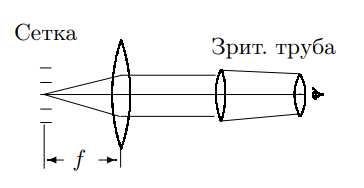
\includegraphics[width=1\linewidth]{plus_lens.PNG}
\caption{Определение фокусного расстояния собирающей линзы} %% подпись к рисунку
\label{ris:experimoriginal} %% метка рисунка для ссылки на него
\end{minipage}
\hfill 
\begin{minipage}[h]{0.40\linewidth}
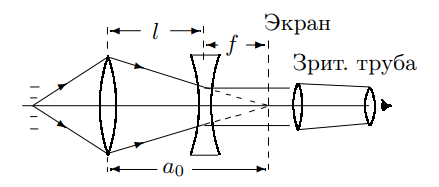
\includegraphics[width=1\linewidth]{minus_lens.PNG}
\caption{Определение фокусного расстояния рассеивающей линзы}
\label{ris:experimcoded}
\end{minipage}
\end{center}
\end{figure}

\newpage %%%%%%%%%%%%%%%%%%%%%%%%%%%%%%%%%%%%%%%%%%%%%%%%%



\subsection{Телескоп Кеплера}

В качестве коллиматора использовалась линза 3 (с фокусным расстоянием ~20см), для телескопа были выбраны линзы 2 и 4, чтобы предполагаемое увеличения было между 2 и 3. Расстояние между объективом и окуляром телескопа после настройки было равно $39.4 \pm 0.2 \simeq 39 \pm 0.4$. Рассчитанное угловое увеличение $$N_{T}=-\frac{f_{1}}{f_{2}}=2.54 \pm 0.06.$$

В то же время угловое увеличение можно определить через отношение углов, под которыми видно деление сетки с трубой и без нее. Для этого в делениях шкалы зрительной трубы определим $h_{1} = 9 \pm 1$ у.е. размер деления шкалы без трубы и $h_{2} = 24 \pm 2$ с трубой Кеплера. В силу того что $h \approx k \alpha$, где $k$ - некоторый коэффициент увеличения зрительной трубы, получаем что $$N_{T}=\frac{\alpha_{2}}{\alpha_{1}}=\frac{h_{2}}{h_{1}}=2.66 \pm 0.4.$$

Еще один способ рассчитать увеличение телескопа - через отношение диаметров пучка, прошедшего через объектив, и пучка, вышедшего из окуляра:
$$N_{T}=-\frac{D_{1}}{D_{2}}=2.77 \pm 0.29.$$

В целом можно заметить что все три способа дают приблизительно равные результаты (в пределах погрешности). Наименее доверительным может показать последний способ, что естественно, так как определение диаметра круговых объектов линейкой трудно выполнить хорошо.

\subsection{Труба Галилея}
Для сборки трубы галилея окуляр был заменен на рассеивающую линзу (на расстоянии от объектива равному разности модулей фокуса объектива и окуляра). Соответственно расчетное увеличение было равно
$$N_{T}=-\frac{f_{1}}{f_{2}}=3.11 \pm 0.11.$$

А из расчета через увеличения размера изображения в зрительной трубе:
$$N_{T}=\frac{\alpha_{2}}{\alpha_{1}}=\frac{h_{2}}{h_{1}}=3 \pm 0.55.$$

Опять же, расчет увеличения обоими способами совпал. Способ через размер видимого изображения решетки опять дал значение с высокой погрешностью. Это объясняется во-первых, тем что толщина прутьев увеличенной решетки превышала точность шкалы зрительной трубы, а во-вторых, колебаниями установки, из-за чего изображение "тряслось" и вносилась дополнительная погрешность.


%%%%%%%%%%%%%%%%%%%%%%%%%%%%%%%%%%%%%%%%%%%%%%%%%%%%%%%%%%%%%%%%%%%%%%%%%

\subsection{Микроскоп}
Планируемое увеличение микроскопа было принято равным $N_{M} = 5$. С учетом формул
$$
N_{M}=N_{1} N_{2}, \quad N_{1}=-\frac{\Delta}{f_{1}}, \quad N_{2}=\frac{L}{f_{2}}, \quad \Delta=\ell_{12}-f_{1}-f_{2}
$$
были расчитаны оптический интервал $\Delta = 17.6 \pm 0.8$ см и длина тубуса $\ell_{12} = 36.6 \pm 1.2$ см. Увеличение микроскопа было определено по увеличению изображения деления сетки ($h_{2} = 32 \pm 2$ см):
$$
N_{M}=-\frac{h_{2}}{h_{1}} \frac{L}{f} = 5.4 \pm 0.7
$$
Как видно, рассчитанное увеличение попадает в предполагаемый интервал в пределах погрешности. При этом вклад причин, вносящих погрешность в расчет, которые были упомянуты в пункте про трубу Галилея увеличивается, так как увеличивается сам размер изображения в зрительной трубе.
\section{Выводы}
\begin{enumerate}
    \item Были определены фокусные расстояния линз из набора, одна из которых была рассеивающей
    \item Были сконструированы модели таких оптических систем как труба кеплера, труба Галилея и микроскоп. Для всех были экспериментально определены увеличения, совпавшие с рассчитанными теоретически

\end{enumerate}

\end{document}
